% AI 论文
% twocolumn 代表的是 两栏的内容ctexart
% ctexart article会build不通过
\documentclass[UTF8,twocolumn, a4paper]{ctexart}
\usepackage{CJK}
\setlength\textwidth{8cm}
\setlength\textheight{8cm}

% 调用包

\usepackage{ctex}
% 数学公式
\usepackage{amsmath}
\usepackage{amssymb}%花体字符

\usepackage[left=2.50cm,right=2.50cm,top=2cm,bottom=2cm]{geometry}
%% 美国数学学会包
\usepackage{amssymb,amsfonts,amsmath,amsthm}

% figure
% \usepackage{graphicx}
% \usepackage{subfigure}
\usepackage{graphics}

% 自绘图
\usepackage{tikz}
\usepackage{chngpage}

% 宏包fancyhdr: 来设定文章的页眉页脚
\usepackage{fancyhdr}

\title{A*算法在UAV中的应用}
\author{fengxuewei}
\date{\today}

\pagestyle{fancy}

% 由于里面没有任何参数,所以这条命令用来清空所有的页眉设置。
\fancyhead{}
% 清除页脚设置
\fancyfoot{}
\fancyhead[L]{\slshape {A*算法在UAV中的应用}}
\fancyhead[R]{\slshape 冯学伟}
\fancyfoot[C]{\thepage}

\renewcommand{\refname}{参考文献}
\usepackage[numbers,sort&compress,super,square]{natbib}
\begin{document}

    % \maketitle
    % \begin{abstract}
    % 1. 将RC和offboard控制指令综合调用 \\
    % 2. RC 产生 yaw 的值, offboard 的 position control 产生的是 throttle, pitch, roll 的值\\
    % 3. 四者进行结合, 更好的控制UAV
    % \end{abstract}

    % 正文中只有使用了\maketitle后才会出现插入的内容 
    % 显示 title author date
    \maketitle

    % 目录
    \tableofcontents % 插入目录
    \thispagestyle{empty} % 设置当前页 页版式
    \clearpage % 插入新的一页
    
    
    \begin{center}
    \large{\textbf{摘要}}
    \end{center}
    \begin{abstract}{1cm}{1cm}
        摘要的内容(中英文, 关键词)\\
        这里是中文摘要。这里是中文摘要。这里是中文摘要。这里是中文摘要。这里是中文摘要。这里是中文摘要。这里是中文摘要。这里是中文摘要。这里是中文摘要。这里是中文摘要。这里是中文摘要。这里是中文摘要。这里是中文摘要。这里是中文摘要。这里是中文摘要。这里是中文摘要。
        
        这里是中文摘要。这里是中文摘要。这里是中文摘要。这里是中文摘要。这里是中文摘要。这里是中文摘要。这里是中文摘要。这里是中文摘要。这里是中文摘要。这里是中文摘要。这里是中文摘要。这里是中文摘要。这里是中文摘要。这里是中文摘要。这里是中文摘要。
    \end{abstract}    
    \clearpage % 插入新的一页

    \begin{center}
    \large{\textbf{Abstract}}
    \end{center}

    \begin{adjustwidth}{1cm}{1cm}
    \hspace{1.5em}Here is the first par. of abstract.Here is the first par. of abstract.Here is the first par. of abstract.Here is the first par. of abstract.Here is the first par. of abstract.Here is the first par. of abstract.Here is the first par. of abstract.Here is the first par. of abstract.Here is the first par. of abstract.Here is the first par. of abstract.Here is the first par. of abstract. 
    \noindent\hspace{1.5em}Here is the second par. of abstract.Here is the second par. of abstract.Here is the second par. of abstract.Here is the second par. of abstract.Here is the second par. of abstract.Here is the second par. of abstract.Here is the second par. of abstract.Here is the second par. of abstract.
    \end{adjustwidth}
    \clearpage % 插入新的一页
        
    \section{引言}
        % 加上 \ 让其当做一个logo进行排版
        \LaTeX 是一个比较好用的排版平台,但是入门比较困难,相比较word而言,但是排版比较大的文件,不会死机,并且可以多人分工合作,采用一样的模板,主要用在数学、物理教材可以用。作图可以用figure这个包,把文件路径引进来就可以了。

        \LaTeX 的入门相对困难一些,这个系统平台的安装包也比较大,一般接近3G的大小。百度搜索CTex,中科院的有个博士论文包,可以参考学习。
        可以排版优美的数学公式。
    \section{数学公式的排版}
        数学公式的排版,我们要掌握latex语言,比较繁琐,不过可以mathtype导出TeX代码,也可以手写图片,采用mathpix snipping tools,识别率到90\%。

        % 将公式单独列为一行
        % gather* 下面的公司不会产生 编号; 
        % gather 会产生编号
        % \\ 代表的是换行
        \begin{gather*}
            f(x) = x ^ 2 \\
            f(x) = x_1^2 + {x}_{2}^{2}
        \end{gather*}
        数学公式分为二种,一种叫做行内公式,$v=v_0+at$,
        还有一种叫做块状公式,
        \[
            x=v_0 t+\frac{1}{2} at^2   
        \]
        带编号的公式
        % 多行公式 gather输入的好处是每一行,他都会按照前文的编号计数器进行向下计数,这样保证了公式编号的连贯性。
        \begin{gather}%会产生编号
            a+b=b+a\\
            ab=ba
        \end{gather}
         
        \begin{gather*}%不会产生编号
            % \times 表示 乘号
        a \times b=b \times a\\
        ab=ba   
        \end{gather*}
         
        \begin{gather}%会编号
        a+b=b+a \notag \\%\notag阻止编号
        ab=ba   \notag %\notag阻止编号
        \end{gather}
         
         
         
        %align和align*环境(用$对齐)
        % * 有无的区别只是针对编号的有无
        \begin{align}
            x &= t + \cos t + 1\\
            y &= 2\sin t
        \end{align}
           %split环境(用$对齐)(一个公式分为多行排版)
        \begin{equation}
            \begin{split}
            \cos 2x &= \cos^2 x - \sin^2 x\\
            &= 2\cos^2 x - 1
            \end{split}
        \end{equation}
         
         
        %case环境
        %每行公式使用&分割成两部分
        %通常表示值和后面的条件
        \begin{equation}
            D(x) = \begin{cases}
            1, &\text{如果} x \in \mathbb{Q}\\%mathbb花体字符
            0, &\text{如果} x \in \mathbb{R}\setminus\mathbb{Q}	
                   \end{cases}%\text是为了在数学公式中处理中文
        \end{equation}
         

        \begin{equation}%%% equation环境,可以自动编号
            \nabla \cdot E =\frac{\rho_0}{\varepsilon_0}
        \end{equation}
        多个公式采用一个编号
        % \frac{分子}{分母}
        \begin{equation}
            \begin{split}
                % \frac{x_2^2}{x_0^3}\\
                \nabla \cdot E &=\frac{\rho_0}{\varepsilon_0}\\
                \nabla \times E&=0  ~~~~    \text{麦克斯韦方程组}
            \end{split}
        \end{equation}
        测试一下

    \section{图片的制作}
    % 子标题的插入
    \subsection{figure包下的图片引入}
        % \usepackage{graphicx}和\usepackage{subfigure}
        % \begin{figure}
        %     \centerline{helloworld}
        %     \centering % 图片居中
        %     % 指定图像的大小
        %     % \includegraphics[属性]{相同文件下的图片名字}
        %     % 属性: 
        %     %       width=3in 设定图片的大小为 3 inches
        %     %       width=\testwidth 设定图片大小的为文本宽度。
        %     %       width=0.3\textwidth 文本宽度的 0.3 倍
        %     %       width=\testwidth-2.0in 比文本宽度 少 2.0 inches

        %     %       angle=270 将图片旋转270度
        %     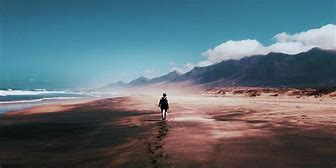
\includegraphics[width=0.2\textwidth, angle=45]{OIP.jpg}
        %     \caption{摩擦角}
        %     \label{fraction}
        % \end{figure}
        % \ref{fraction} 生成引用
        % 根据图(\ref{fraction}),图片引入方式,这是位图,也可以pdf,也可以是eps。
    \subsection{tikz图片的生成}
    \begin{tikzpicture}
        \draw (0,0) circle (3cm);
        \draw (6,0) rectangle (12,2);
    \end{tikzpicture}
    推荐学习的网站LaTeX Studio,这个网站有很多教程,也有很多模板,tikz网站也有很多模板,自己尝试着去改。


% \cite{author1.year1,author2.year2}
% “99” 表示以最多两位数来编号参考文献, 用于对齐
\begin{thebibliography}{99}
\addtolength{\itemsep}{-2ex} % 用于更改行距
\bibitem{author1.year1}Au1. ArtName1[J]. JN1. Y1:1--2
\bibitem{author2.year2}Au2. ArtName2[J]. JN2. Y2:1--2
\end{thebibliography}    
    

\end{document}
